\chapter{Results}\label{cap:results}

\section{Multiple Linear Regression Model and Regression Tree Model}

%O primeiro experimento definido para este trabalho é estabelecer uma linha de base para que seja possível comparar o desempenho de outras abordagens com a base de dados selecionada. Inicialmente, esse experimento consiste na seleção entre MRLM e MAR como linha de base. Isso pode ser realizado após discutir a informação apresentada na Tabela \ref{tab:lm_descriptive} e na Figura \ref{fig:mlrm_result}.
The first experiment set for this work is to establish a baseline so that you can compare the performance of alternative approaches to the selected database. Initially, this experiment consists of selecting among MLRM and RTM as a baseline. This can be done after discussing the information presented in Table \ref{tab:lm_descriptive} and Figure \ref{fig:mlrm_result}.

Table \ref{tab:lm_descriptive} shows descriptive statistics of normalized RMSE's to both algorithms. Average, standard deviation, minimum and maximum values are calculated for one MLRM and three RTM: $MLRM$ (cv.lm.v1), $RTM_1$ (cv.rpart.v1), $RTM_2$ (cv.rpart.v2) and $RTM_3$ (cv.rpart.v3).
%A Tabela \ref{tab:lm_descriptive} mostra a estatística descritiva do REMQ normalizado para ambos os algoritmos. Os valores de média, desvio padrão, mínimo e máximo são calculados para um Modelo de Regressão Linear Múltipla e três Modelos de Regressão em Árvore: MRLM (cv.lm.v1), $MRA_1$ (cv.rpart.v1), $MRA_2$ (cv.rpart.v2) and $MRA_3$ (cv.rpart.v3).

\begin{table}[h]
\caption{Descriptive statistics for normalized errors of linear regression models.}\label{tab:lm_descriptive} \centering
\begin{tabular}{|c|c|c|c|c|}
  \hline
   & $MLRM$ & $RTM_1$ & $RTM_2$ & $RTM_3$ \\
  \hline
  Average & \textbf{0.09912} & 0.10238 & 0.10305 & 0.10361  \\
  \hline
  Std Dev & \textbf{0.00391} & 0.00423 & 0.00441 & 0.00426  \\
  \hline
  Min. & \textbf{0.08956} & 0.09214 & 0.09321 & 0.09372  \\
  \hline
  Max. & \textbf{0.10746} & 0.11231 & 0.11267 & 0.11359  \\
  \hline
\end{tabular}
\end{table}

\begin{figure}[h]
  \vspace{-0.2cm}
  \centering
  \includegraphics[width=\columnwidth]{image/mrl_ex1.pdf}
  \caption{Boxplots for normalized errors of linear regression models.}
  \label{fig:mlrm_result}
\end{figure}

In Figure \ref{fig:mlrm_result}, normalized RMSE's boxplots after predictions for $RTM_3$, $RTM_2$, $RTM_1$ and MLRM are presented. The minor RMSE is obtained in MLRM, this regression model also has minor standard deviation. From those information, we can affirm MLRM is a more efficient and precise model and will be introduced in the experiment as baseline method.
%Na Figura \ref{fig:mlrm_result}, os \textit{boxplots} da REMQ normalizado após as previsões para MRLM, $MRA_1$, $MRA_2$ e $MRA_3$ são apresentados. O menor REMQ é obtido para o MRLM, esse modelo de regressão também tem menor desvio padrão. A partir dessa informação, pode-se afirmar que o MRLM é um modelo eficiente e preciso e é definido como modelo de linha de base.

\section{Monte Carlo Simulation and PERT Analysis}

%O segundo experimento é analisar o desempenho das técnicas convencionais utilizadas na academia e na indústria, inclusive determinadas como boas práticas pelo PMBOK \cite{PMBOK2008}. Como explicado anteriormente, essas abordagens foram configuradas para obterem o melhor desempenho possível.
The second experiment is to analyze the performance of conventional techniques used in academia and industry, including best practices as determined by PMBOK \cite{PMBOK2008}. As explained earlier, these approaches have been configured to obtain the best possible performance.

%A Tabela \ref{tab:arte_descriptive} mostra a estatística descritiva do REMQ normalizado para ambos os algoritmos. Os valores de média, desvio padrão, mínimo e máximo, calculados para Simulação de Monte Carlo e para a Análise PERT, mostram que a Análise PERT apresenta valores bem inferiores de média, mínimo e máximo. No entanto, o desvio padrão da Simulação de Monte Carlo é menor, provando ser um método mais preciso.
Table \ref{tab:arte_descriptive} shows the descriptive statistics for normalized RMSE for both algorithms. The mean value, standard deviation, minimum and maximum, calculated for Monte Carlo Simulation and PERT Analysis, presents that the PERT Analysis has lower mean, minimum and maximum values. However, MCS has lower standard deviation, proving to be more precise between than.

\begin{table}[h]
\caption{Descriptive statistics for normalized errors of state of art models.}\label{tab:arte_descriptive} \centering
\begin{tabular}{|c|c|c|}
  \hline
   & MCS & PERT \\
  \hline
  Average & 0.12640 & \textbf{0.07466}   \\
  \hline
  Std. Deviation & \textbf{0.01250} & 0.01438   \\
  \hline
  Minimum & 0.10410 & \textbf{0.04788}   \\
  \hline
  Maximum & 0.14950 & \textbf{0.09122}   \\
  \hline
\end{tabular}
\end{table}

\begin{figure}[h]
  \vspace{-0.2cm}
  \centering
  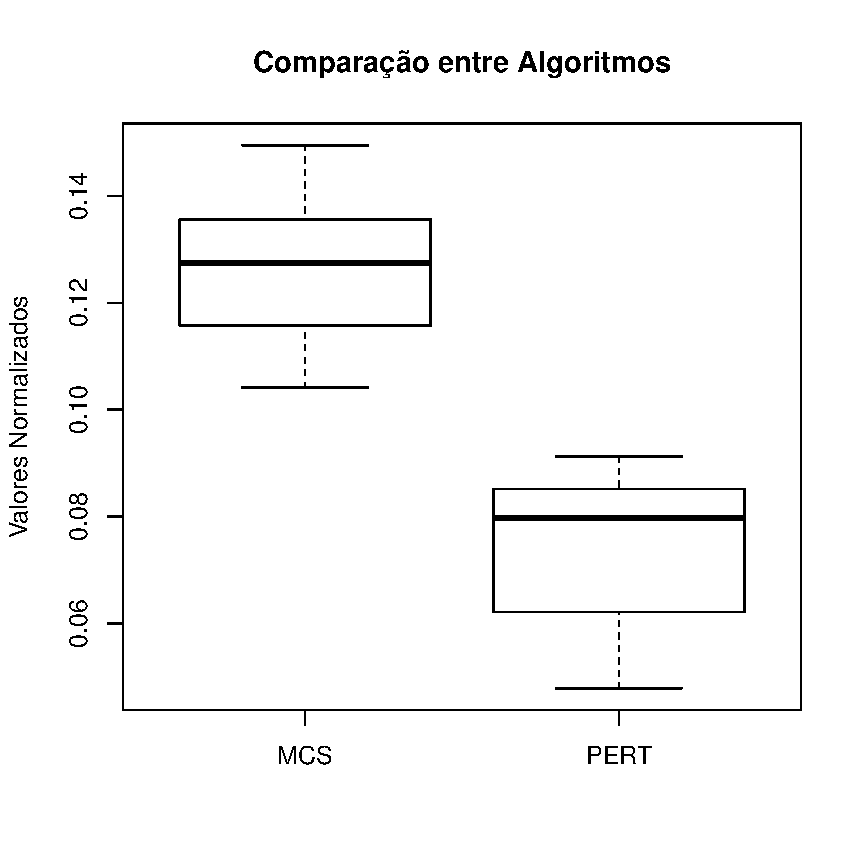
\includegraphics[trim = 1mm 12mm 1mm 1mm,clip,width=0.7\columnwidth]{image/arte_ex2.pdf}
  \caption{Boxplots for normalized errors of linear regression models.}
  \label{fig:arte_result}
\end{figure}

%Na Figura \ref{fig:arte_result}, os \textit{boxplots} da REMQ normalizado após as previsões para SMC e PERT são apresentados. A partir dessa informação, pode-se afirmar que a Análise PERT é um modelo de estado da arte mais eficiente e ligeiramente preciso, nessa comparação.
In Figure \ref{fig:arte_result}, the boxplots of normalized RMSE after forecasts for MCS and PERT are presented. From this information, it can be stated that PERT Analysis is a more efficient state of art and slightly more precise, in this comparison.

%A Análise PERT mostrou ser uma abordagem bastante interessante quando há poucas informações de riscos nas lições aprendidas no gerenciamento de projetos anteriores, como uma base de dados de registro de riscos. Uma análise detalhada utilizando uma base de dados revela que essa técnica apresenta resultados aceitáveis pelos gerentes de projetos.
PERT analysis proved to be a very interesting approach when is little risk information in learned lessons of previous projects, such as a risk register database. A detailed analysis using a database reveals that this technique has acceptable results to project managers.

\section{MultiLayer Perceptron and variations}

%Nesse experimento, algumas MLPs foram avaliadas. A principal diferença entre elas é a regra de aprendizagem. Os algoritmos: \textit{Backpropagation}, Levenberg-Marquardt, Broyden-Fletcher-Goldfarb-Shanno \textit{Backpropagation}, Gradiente Conjugado Escalonado, \textit{Resilient-propagation}, \textit{Resilient-propagation}, \textit{One-step Secant backpropagation} e Quasi-Newton foram alguns dos selecionados.
In this experiment, some MLPs were assessed. The main difference between than is the learning rule; Backpropagation, Levenberg-Marquardt, Broyden-Fletcher-Goldfarb-Shanno Backpropagation, Scaled Conjugate Gradient, Resilient-propagation, One-step Secant backpropagation and Quasi-Newton algorithms sre some of them selected.

%Na Tabela \ref{tab:mlps_descriptive}, é exibida a estatística descritiva do REMQ normalizado para as abordagens desenvolvidas para esse experimento. Os valores de média, desvio padrão, mínimo e máximo são calculados para cada uma das MLPs. "BP" apresenta os resultados para uma MLP com algoritmo de aprendizagem \textit{Backpropagation}; "LM" para uma MLP com o algoritmo Levenberg-Marquardt; "BFGS" para uma MLP com o algoritmo Broyden-Fletcher-Goldfarb-Shanno \textit{Backpropagation}; "SCG" para uma MLP com o algoritmo Gradiente Conjugado Escalonado; "RP" para uma MLP com o algoritmo \textit{Resilient-propagation}; "RPCG" para uma MLP com o algoritmo \textit{Resilient-propagation} combinado com o Gradiente Conjugado; "OSS" para uma MLP com o algoritmo \textit{One-step Secant backpropagation}; por fim, "Reg" para uma MLP chamada "MLPRegressor" com o algoritmo BFGS Quasi-Newton. Conforme os valores médio, mínimo e máximo, observa-se que a alternativa "Reg" é mais eficiente, mesmo tendo o maior desvio padrão segundo esse experimento.
Table \ref{tab:mlps_descriptive} shows off descriptive statistics of normalized RMSE to approaches developed for this experiment. The mean, standard deviation, minimum and maximum values are calculated for each of the MLPs. "BP" shows results for a MLP with backpropagation learning algorithm; "LM" for an MLP with Levenberg-Marquardt algorithm; "BFGS" for an MLP with Broyden-Fletcher-Goldfarb-Shanno Backpropagation algorithm; "SCG" for an MLP with Scaled Conjugate Gradient algorithm; "RP" for an MLP with Resilient-propagation algorithm; "RPCG" for an MLP with Resilient-propagation combined with Conjugate Gradient algorithm; "OSS" for an MLP with One-step Secant backpropagation algorithm. Finally, "Reg" for an MLP called "MLPRegressor" with the BFGS Quasi-Newton algorithm. According to average, minimum and maximum values, it is observed that "Reg" is a more efficient alternative, even with the largest standard deviation second this experiment.

\begin{table}[h]
\caption{Descriptive statistics for normalized errors of MLPs models.}\label{tab:mlps_descriptive} \centering
\begin{tabular}{|c|c|c|c|c|c|c|c|c|}
  \hline
   & BP & LM & BFGS & SCG & RP & RPCG & OSS & Reg \\
  \hline
  Avg & 0.1000 & 0.0986 & 0.0980 & 0.0982 & 0.0979 & 0.0981 & 0.0995 & \textbf{0.0516}   \\
  \hline
  StD & 0.0015 & 0.0018 & \textbf{0.0011} & 0.0018 & 0.0015 & 0.0021 & 0.0031 & 0.0042   \\
  \hline
  Min & 0.0973 & 0.0952 & 0.0945 & 0.0951 & 0.0946 & 0.0950 & 0.0943 & \textbf{0.0427}   \\
  \hline
  Max & 0.1041 & 0.1035 & 0.1004 & 0.1037 & 0.1019 & 0.1041 & 0.1065 & \textbf{0.0603}   \\
  \hline
\end{tabular}
\end{table}

\begin{figure}[h]
  \vspace{-0.2cm}
  \centering
  \includegraphics[trim = 1mm 10mm 1mm 1mm,clip,width=\columnwidth]{image/mlps_ex3.pdf}
  \caption{Boxplots for normalized errors of multiple linear perceptron networks.}
  \label{fig:mlps_result}
\end{figure}

%Na Figura \ref{fig:mlps_result}, os \textit{boxplots} da REMQ normalizado após as previsões para as oito MLPs são apresentados. A partir dessas informações, pode-se afirmar que a MLP chamada "MLPRegressor" é uma rede neural mais eficiente porém aidna imprecisa, de acordo com o experimento.
In Figure \ref{fig:mlps_result}, boxplots of normalized RMSE after forecasts for the eight MLPs are presented. From this information, it can be stated that a MLP called "MLPRegressor" is a more efficient but still imprecise artificial neural network, according to experiment.

\section{MLP, SVM, RBF and ANFIS}

%Após avaliar uma rede neural eficiente no experimento anterior, o quarto experimento tem o objetivo de eleger qual a melhor técnica baseada em Redes Neurais Artificiais, dentre as implementadas, para a previsão do impacto de riscos a partir da base de dados PERIL.
After evaluating an efficient neural network in the previous experiment, the fourth experiment aims to elect the best technique based on Artificial Neural Networks, among implemented for predicting risk impact from PERIL database.

%A Tabela \ref{tab:anns_descriptive} mostra a estatística descritiva do REMQ normalizado para as RNAs estudadas. Os valores de média, desvio padrão, mínimo e máximo, calculados para um modelo Neuro-Fuzzy ANFIS, uma SVM (chamada SMORegressor), uma rede RBF (chamada RBFRegressor) e para uma "MLPRegressor" mostram que o último algoritmo apresenta valores bem inferiores de média, mínimo e máximo. No entanto, o desvio padrão do ANFIS é menor. Portanto, "MLPRegressor" prova ser um método mais eficiente e relativamente preciso, em comparação com as outras técnicas, para a estimativa do impacto de risco baseada na PERIL.
Table \ref{tab:anns_descriptive} shows the descriptive statistics for the normalized RMSE to studied ANNs. The mean, standard deviation, minimum and maximum value calculated for a Neuro-Fuzzy model ANFIS, an SVM (called SMORegressor), an RBF network (called RBFRegressor) and for a "MLPRegressor" show that the latter algorithm has much lower average, minimum and maximum values. However, the standard deviation of ANFIS is lower. Therefore, "MLPRegressor" proves to be a relatively efficient and accurate method compared with other techniques to risk impact estimation based on PERIL.

\begin{table}[h]
\caption{Descriptive statistics for normalized errors of ANNs models.}\label{tab:anns_descriptive} \centering
\begin{tabular}{|c|c|c|c|c|}
  \hline
   & ANFIS & SMOReg & RBFReg & MLPReg  \\
  \hline
  Avg & 0.1079 & 0.09430 & 0.09004 & \textbf{0.0516}   \\
  \hline
  StD & \textbf{0.00003} & 0.00488 & 0.00432 & 0.0042   \\
  \hline
  Min & 0.1078 & 0.08347 & 0.08024	 & \textbf{0.0427}   \\
  \hline
  Max & 0.1080 & 0.10284 & 0.09790 & \textbf{0.0603}   \\
  \hline
\end{tabular}
\end{table}

\begin{figure}[!h]
  \vspace{-0.2cm}
  \centering
  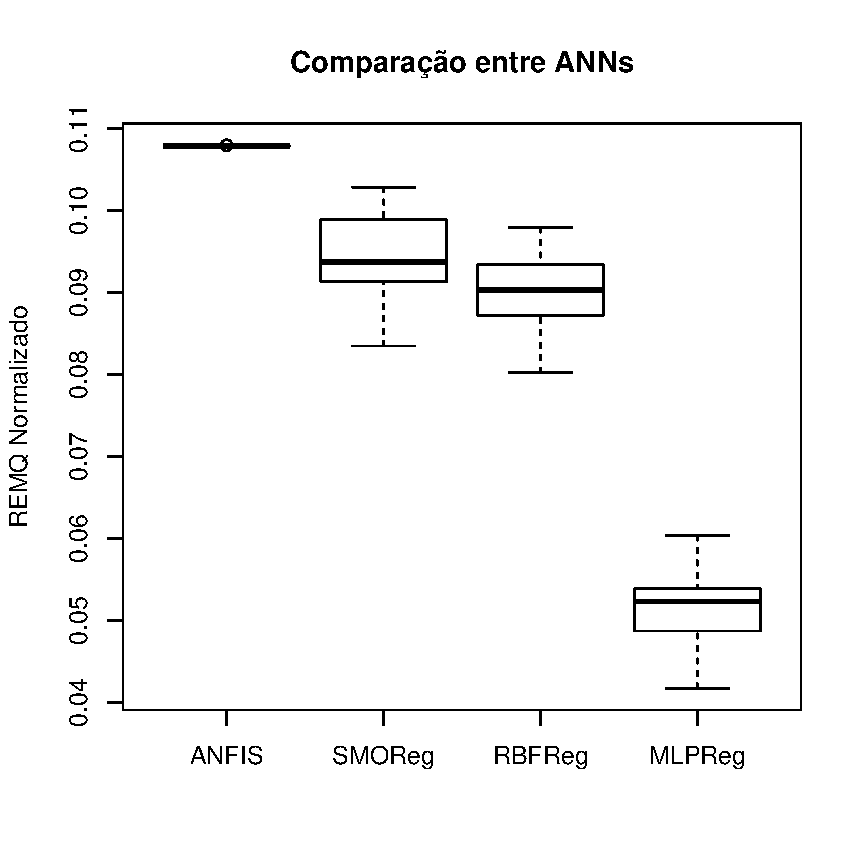
\includegraphics[trim = 1mm 12mm 1mm 1mm,clip,width=0.7\columnwidth]{image/anns_ex4.pdf}
  \caption{Boxplots for normalized errors of ANNs.}
  \label{fig:anns_result}
\end{figure}

%Na Figura \ref{fig:anns_result}, os \textit{boxplots} da REMQ normalizado após as estimativas de impacto das RNAs são apresentados. A partir dessas informações, pode-se afirmar que o "MLPRegressor" é uma Rede Neural Artificial mais eficiente e ligeiramente precisa, de acordo com essa comparação.
In Figure \ref{fig:anns_result}, boxplots of normalized RMSE after impact prediction of RNAs are shown. From this information, it can be stated that the "MLPRegressor" is a more efficient Artificial Neural Network and slightly accurate, according to this comparison.

\begin{figure}[!h]
  \centering
  
\includegraphics[trim = 1mm 12mm 1mm 8mm,clip,width=\columnwidth]{image/epocas.png}
  \caption{Convergence of ANFIS.}
  \label{fig:anns_result_2}
\end{figure}

%Na Figura \ref{fig:anns_result_2}, é apresentada a convergência do ANFIS, em termos da REMQ normalizado, para cada época durante o treinamento até ser interrompido, de acordo com a validação cruzada. Observa-se que o algoritmo encontra um mínimo local e permanece preso até o treinamento ser interrompido. Logo, conclui-se que o ANFIS apresenta algumas limitações de convergência para essa base de dados.
In Figure \ref{fig:anns_result_2}, the convergence of ANFIS is presented in terms of normalized resched for each season during training to be stopped, according to cross-validation. It is observed that the algorithm finds a local minimum and remains stuck until stopping the training. Therefore, it is concluded that the ANFIS has some limitations on convergence for this database.

\begin{figure}[!h]
  \vspace{-0.2cm}
  \centering
  \includegraphics[trim = 1mm 12mm 1mm 1mm,clip,width=0.7\columnwidth]{image/smoreg_ex4.pdf}
  \caption{Boxplots for normalized errors of SVM.}
  \label{fig:anns_result_5}
\end{figure}

%Na Figura \ref{fig:anns_result_5}, os \textit{boxplots} dos impactos esperados e calculados pelo algoritmo "SMORegressor" de cinqunta amostras são apresentados. O resultado ideal é que os \textit{boxplots} das duas amostras sejam o mais semelhantes possível, respeitando a mediana, o intervalo inter-quartil e os valores de mínimo e máximo. A partir da informação apresentada, pode-se concluir que o \textit{boxplot} oriundo dos impactos calculados tenta representar mas distorce em todas as medidas os impactos esperados.
In Figure \ref{fig:anns_result_5}, boxplots of expected and calculated impacts of fifth samples by "SMORegressor" algorithm are presented. The ideal result is boxplots of both samples being as similar as possible, respecting median, interquartile range, minimum and maximum values. From the information presented, it can be concluded that boxplot coming from calculated impacts attempts to represent but distorts in all measures the expected impacts.

\begin{figure}[!h]
  \vspace{-0.2cm}
  \centering
  \includegraphics[width=0.7\columnwidth]{image/smoreg_ex4_2.pdf}
  \caption{Normalized errors of expected and calculated impacts.}
  \label{fig:anns_result_6}
\end{figure}

%Na Figura \ref{fig:anns_result_6}, as cinquenta primeiras amostras do subconjunto de testes e da saídas calculadas são apresentadas, graficamente. A partir desses gráficos, pode-se observar que o algoritmo "SMORegressor" tem dificuldade em estimar os resultados esperados, quase não apresentando relação com eles.
In Figure \ref{fig:anns_result_6}, the first fifty samples of expected and calculated outputs are presented graphically. From these graphs, it can be observed that the "SMORegressor" algorithm has difficulty in estimating the expected results, showing almost no relationship with the last ones.

\begin{figure}[!h]
  \vspace{-0.2cm}
  \centering
  \includegraphics[trim = 1mm 12mm 1mm 1mm,clip,width=0.7\columnwidth]{image/rbfreg_ex4.pdf}
  \caption{Boxplots for normalized errors of RBF networks.}
  \label{fig:anns_result_3}
\end{figure}

%Na Figura \ref{fig:anns_result_3}, os \textit{boxplots} dos impactos esperados e calculados pelo algoritmo "RBFRegressor" de cinquenta amostras são apresentados. O resultado ideal é que os \textit{boxplots} das duas amostras sejam o mais semelhantes possível, respeitando a mediana, o intervalo inter-quartil e os valores de mínimo e máximo. A partir da informação apresentada, pode-se concluir que o \textit{boxplot} oriundo dos impactos calculados tenta representar mas distorce no quartil inferior e nos valores máximos os impactos esperados.
In Figure \ref{fig:anns_result_3}, the boxplots of expected and calculated impacts by "RBFRegressor" of fifth samples are presented. The ideal result is that boxplots of both samples are as similar as possible, respecting the median, interquartile range, minimum and maximum values. From the information presented, it can be concluded that boxplots coming from the calculated impacts attempts but distorts to represent the lower quartile and maximum values of expected impacts. 

\begin{figure}[!h]
  \vspace{-0.2cm}
  \centering
  \includegraphics[width=0.7\columnwidth]{image/rbfreg_ex4_2.pdf}
  \caption{Normalized errors of expected and calculated impacts.}
  \label{fig:anns_result_4}
\end{figure}

%Na Figura \ref{fig:anns_result_4}, as cinquenta primeiras amostras do subconjunto de testes e da saídas calculadas são apresentadas, graficamente. A partir desses gráficos, pode-se observar que o algoritmo "RBGRegressor" tem dificuldade em estimar os resultados esperados, principalmente os valores máximos e mínimos.
In Figure \ref{fig:anns_result_4}, the first fifty samples of test subset and calculated outputs are presented graphically. From these graphs, it can be observed that the "RBFRegressor" algorithm has difficulty in estimating the expected outcomes, mainly the maximum and minimum values.

\begin{figure}[!h]
  \vspace{-0.2cm}
  \centering
  \includegraphics[trim = 1mm 12mm 1mm 1mm,clip,width=0.7\columnwidth]{image/mlpreg_ex4.pdf}
  \caption{Boxplots for normalized errors of expected and calculated outcomes for MLPRegressor.}
  \label{fig:anns_result_7}
\end{figure}

%Na Figura \ref{fig:anns_result_7}, os \textit{boxplots} dos impactos esperados e calculados pelo algoritmo "MLPRegressor" de cinquenta amostras são apresentados. O resultado ideal é que os \textit{boxplots} das duas amostras sejam o mais semelhantes possível, respeitando a mediana, o intervalo inter-quartil e os valores de mínimo e máximo. A partir da informação apresentada, pode-se concluir que o \textit{boxplot} oriundo dos impactos calculados representa, porém com distorções principalmente no quartil inferior, os impactos esperados.
In Figure \ref{fig:anns_result_7}, boxplots of expected impacts and calculated of fifty samples through "MLPRegressor" algorithm are presented. The ideal result is that boxplots of the both samples to be as similar as possible, respecting the median, interquartile range, minimum and maximum values. From the information presented, it can be concluded that boxplot coming from the calculated impacts, but with distortions mainly in the lower quartile represents the expected impacts.

\begin{figure}[!h]
  \vspace{-0.2cm}
  \centering
  \includegraphics[width=0.7\columnwidth]{image/mlpreg_ex4_2.pdf}
  \caption{Normalized errors of expected and calculated impacts.}
  \label{fig:anns_result_8}
\end{figure}

%Na Figura \ref{fig:anns_result_8}, as cinquenta primeiras amostras do subconjunto de testes e da saídas calculadas são apresentadas, graficamente. A partir desses gráficos, pode-se observar que o algoritmo "MLPRegressor" tem dificuldade em estimar os resultados esperados, porém tende a acompanhar os resultados.
In Figure \ref{fig:anns_result_8}, the first fifty samples of tests subsets and from calculated outputs are presented graphically. From these graphs, it can be observed that "MLPRegressor" algorithm has difficulty in estimating the expected results, but has approximate tendency.

\section{Better Model Validation}

A Tabela \ref{tab:validacao_descriptive} mostra a estatística descritiva do REMQ normalizado para as RNAs estudadas. Os valores de média, desvio padrão, mínimo e máximo, calculados para um MRLM, uma Simulação de Monte Carlo(SMC), uma Análise PERT(PERT) e para uma MLP "MLPRegressor"(MLPReg) mostram que o último algoritmo apresenta valores inferiores de média, desvio padrão, mínimo e máximo. Portanto, "MLPRegressor" prova ser um método mais eficiente e relativamente preciso, em comparação com as outras técnicas, para a estimativa do impacto de risco baseada na PERIL.
%Table \ref{tab:validacao_descriptive} shows descriptive statistics for the normalized RMSE for studied ANNs. Mean, standard deviation, minimum and maximum values calculated for a MLRM, a Monte Carlo Simulation (MCS), a PERT analysis (PERT) and a MLP "MLPRegressor" (MLPReg) show that the latter algorithm has lower mean, standard deviation, minimum and maximum values. Therefore, "MLPRegressor" proves to be a relatively efficient and accurate method compared with other techniques to estimate risk impact based on PERIL.

\begin{table}[h]
\caption{Descriptive statistics for normalized errors of ANNs models.}\label{tab:validacao_descriptive} \centering
\begin{tabular}{|c|c|c|c|c|}
  \hline
   & MLR & MCS & PERT & MLPReg  \\
  \hline
  Avg & 0.09912 & 0.12640 & 0.07466 & \textbf{0.05168}   \\
  \hline
  StD & 0.00794 & 0.01250 & 0.01438 & \textbf{0.00427}   \\
  \hline
  Min & 0.08956 & 0.10410 & 0.04788	 & \textbf{0.04172}   \\
  \hline
  Max & 0.10746 & 0.14950 & 0.09122 & \textbf{0.06035}   \\
  \hline
\end{tabular}
\end{table}

\begin{figure}[!h]
  \vspace{-0.2cm}
  \centering
  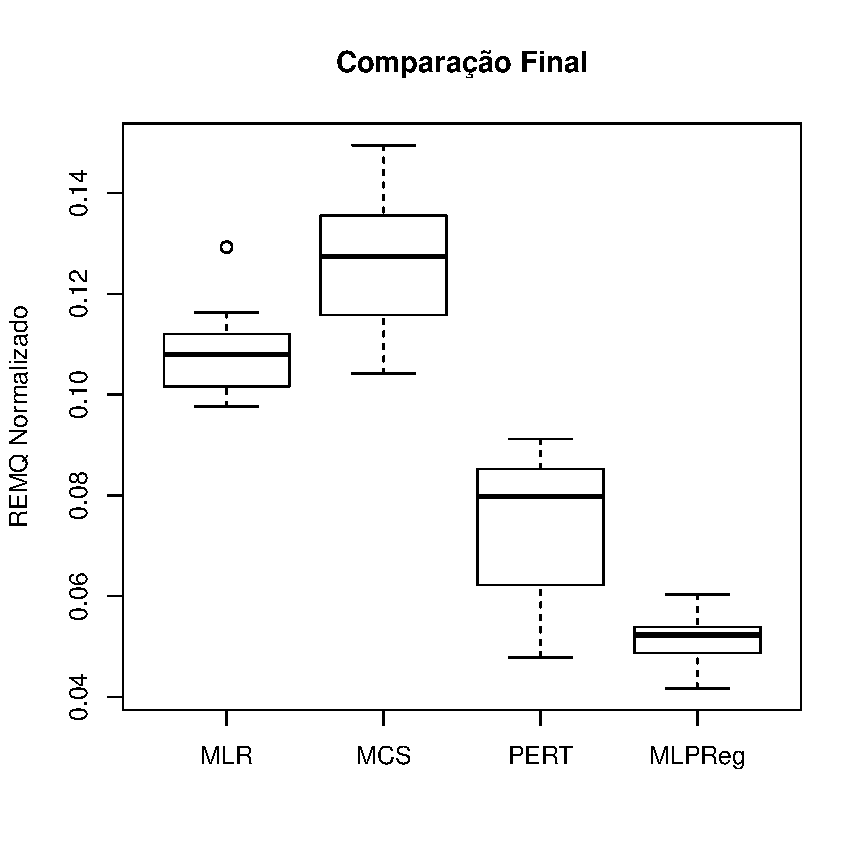
\includegraphics[trim = 1mm 12mm 1mm 1mm,clip,width=0.7\columnwidth]{image/validacao_ex5.pdf}
  \caption{Boxplots for normalized errors of models in validation step.}
  \label{fig:validacao_result}
\end{figure}

%Na Figura \ref{fig:validacao_result}, os \textit{boxplots} da REMQ normalizado após as estimativas de impacto das RNAs são apresentados. A Simulação Monte Carlo(SMC) é imediatamente descartada da análise por apresentar erros maiores que o Modelo de Regressão Linear Múltipla (MLR); a Análise PERT (PERT) apresenta-se como uma abordagem simples e rápida para a estimativa do impacto de riscos, porém como é uma técnica estatística está sujeita a algumas situações que geram maiores erros na estimativa; já, o MLPRegressor (MLPReg) apresenta os menor valores de média, desvio padrão, mínimo e máximo de erro. A partir dessas informações, pode-se afirmar que o "MLPRegressor" é uma Rede Neural Artificial mais eficiente e precisa, comparada com o desempenho das outras RNAs.
In Figure \ref{fig:validacao_result}, boxplots of normalized RMSE after the estimated impact of RNAs are shown. Monte Carlo Simulation (MCS) is immediately discarded from the analysis because it shows higher errors than Multiple Linear Regression Model (MLRM); PERT analysis (PERT) is presented as a simple and fast approach to estimate the risk impact, but as it is a statistical technique is subject to some situations that generate larger errors in the estimation; now, MLPRegressor (MLPReg) presents the lower mean, standard deviation, minimum and maximum error values. From this information, it can be stated that the "MLPRegressor" is an Artificial Neural Network more efficient and accurate compared with the performance of other ANNs and state of art models.

%A Tabela \ref{tab:anns_descriptive} apresenta os resultados dos Testes de Wilcoxon não-pareados para as RNAs estudadas. O símbolo $\Delta$ significa que a técnica à esquerda apresenta melhores resultados que a acima; diferentemente, o símbolo $\nabla$ siginifica que a técnica acima apresenta melhores resultados que à esquerda. Após analisar a tabela, podemos afirmar que a "MLPRegressor" é melhor que a Análise PERT que, por sua vez, é melhor que o Modelo de Regressão Linear Múltipla.
Table \ref{tab: anns_descriptive} presents the results of non-paired Wilcoxon Tests for analyzed ANNs. The symbol $\Delta$ means that the technique on the left shows better results than the above; otherwise, the symbol $\nabla$ simply means that the above technique presents better results than in the left. After analyzing the table, we can see that the "MLPRegressor" is better than the PERT Analysis that, in turn, is better than the Multiple Linear Regression Model.

%Teste de Hipótese
\begin{table}[h]
\caption{Hypothesis Tests for analyzed ANNs.}\label{tab:teste_hipotese} \centering
\begin{tabular}{|c|c|c|c|c|}
  \hline
   & MLR & MCS & PERT & MLPReg  \\
  \hline
  MLR & - & $\Delta$ & $\nabla$ & $\nabla$   \\
  \hline
  MCS & $\nabla$ & - & $\nabla$ & $\nabla$   \\
  \hline
  PERT & $\Delta$ & $\Delta$ & - & $\nabla$   \\
  \hline
  MLPReg & $\Delta$ & $\Delta$ & $\Delta$ & -   \\
  \hline
\end{tabular}
\end{table}

\section{Impact Estimation and Confidence Interval Definition}

%O último experimento consiste na aplicação prática da metodologia proposta nesse estudo, com base no PERIL. Como alguns passos descritos na metodologia foram seguidos nos experimentos anteriores, resta somente a geração de um intervalo de confiança que é a informação compreendida pelos gerentes de projetos, analistas de projetos e de riscos.
The last experiment consists in the practical used of the methodology proposed in this study, based on PERIL. As some steps described in the methodology were conducted in previous experiments, there remains only the generation of a confidence interval that is information understood by project managers and project and risk analysts.

%A aplicação do intervalo de confiança irá determinar a qualidade dos resultados gerados. A partir dos resultados apresentados pelo modelo, será gerado um intervalo que, para uma determinada previsão, terá 95 \% de chances de conter o valor real. Para isso, será utilizado o método de máxima verossimilhança.
The use of the confidence interval will determine the quality of the results generated. From the results shown by the model, will be generated a range that, for a given provision, will be 95 \% chance of containing the true value. For this, maximum likelihood method will be used.

%O método de máxima verossimilhança considera que existem duas fontes de incertezas para um modelo de previsão. O primeiro, o $\sigma_v$, é a variância do ruído, e o segundo, $\sigma_w$, é a variância da incerteza. O $\sigma_v$ representa a variância dos erros gerados pelo conjunto de validação cruzada na fase de treinamento. Esses valores seguem uma distribuição normal e possuem média zero. Já o $\sigma_w$ é referente à variância de incerteza do modelo e é calculada a partir da utilização do modelo para prever os erros gerados pela própria rede.
The maximum likelihood method considers that there are two sources of uncertainty in a forecast model. The first, $\sigma_v$ is the noise variance, and the second, $\sigma_w$, is the variance of uncertainty. The $\sigma_v$ is the variance of the errors generated by the set of cross-validation in the training phase. Those values follow a normal distribution and average to zero. But, $\sigma_w$ refers to the variance of model uncertainty and is calculated from the use of the model to predict the errors generated by the network itself.

%Assume-se que essas duas fontes de erro são independentes. Então o cálculo da variância total do modelo é dado pela Equação \ref{eq:var_intervalo}.
It is assumed that these two sources of error are independent. Then the calculation of the total variance for the model is given by Equation \ref{eq:var_intervalo}.

\begin{equation}
\label{eq:var_intervalo}
\sigma^{2}_{total} = \sigma^{2}_{v} + \sigma^{2}_{w}
\end{equation}

No processo de validação cruzada do modelo, calcula-se o $\sigma_v$ que é a variância dos erros. Para cada entrada do conjunto calcula-se o erro e ao final do processo a média desses erros e extrai-se sua variância usando a Equação \ref{eq:var_validacao}.
%In cross-validation process of the model, it is calculated the $\sigma_v$ that is the variance of errors. For each input in set the error is calculated, at the end of the process the average of these errors is calculated and its variance is obtained using Equation \ref{eq:var_validacao}.

\begin{equation}
\label{eq:var_validacao}
\sigma_v = \frac{1}{n-1} \sum_{n}^{i=1} (Erro_i - \overline{Erro})^2
\end{equation}

%onde, $n$ é a quantidade de valores; $Erro_i$ é o erro referente à entrada i; $\overline{Erro}$ é a média dos erros.
where, $n$ is the number of values; $Erro_i$ is the error correspondent to input $i$; $\overline{Erro}$ is the error average.

%Para calcular o $\sigma_w$, armazena-se is erros para todas as entrada utilizadas no treinamento da rede, incluindo dados de treinamento e validação cruzada. com esses dados devidamente armazenados e normalizados, cria-se um novo modelo, com novos pesos e novas ligações. Esse modelo terá como objetivo, ou seja, valores desejados, os erros gerados pelo modelo anterior. O $\sigma_w$ será calculado utilizando a mesma fórmula utilizada para o $\sigma_v$. A diferença está na quantidade de dados, pois, para o $\sigma_w$ serão utilizados todos os erros de todos os conjuntos, não só o de validação cruzada.
To calculate $\sigma_w$, errors are stored for all utilized inputs in training, including those in cross-validation subset. Since data are stored and normalized, a new model is obtained with new weights and links. This model will have as desired values the errors generated by the previous model. The $\sigma_w$ will be calculated using the same formula used for the $\sigma_v$. The difference is the amount of data because, $\sigma_w$ uses all errors of all subsets, not only the cross-validation.

%Tendo o $\sigma_v$ e $\sigma_w$ calculados, pode-se calcular o $\sigma_total$. Este será utilizado para calcular o intervalo de confiança a partir da Equação \ref{eq:intervalo_confianca}.
Since $\sigma_v$ and $\sigma_w$ are calculated, one can calculate $\sigma_{total}$. This will be used to calculate the confidence interval from Equation \ref{eq:intervalo_confianca}.

\begin{equation}
\label{eq:intervalo_confianca}
x - t * \sigma_total < x < x + t * \sigma_total
\end{equation}

%onde, $x$ é o valor calculado pela rede e $t$ é o valor extraído da tabela de t de Student para o maior grau de liberdade possível para um intervalo de 95\% de chances de conter o valor real, como exibido na Tabela \ref{tab:lm_descriptive}.
where $x$ is the computed outcome by the network and $t$ is the value extracted from the Student's T table to the largest possible degree of freedom for a period of 95 \% chance of containing the true value, as shown in table \ref{tab:lm_descriptive}.

\begin{table}[h]
\caption{A briefing of Student's T table.}\label{tab:t-student} \centering
\begin{tabular}{|c|c|c|c|c|}
  \hline
  \multicolumn{5}{|c|}{$P(t_n \leq x)$}  \\
  \hline
  \textbf{n} & 0,750 & 0,900 & 0,950 & 0,975  \\
  \hline
  30 & 0,683 & 1,310 & 1,697 & 2,042   \\
  \hline
  40 & 0,681 & 1,303 & 1,684 & 2,021   \\
  \hline
  60 & 0,679 & 1,296 & 1,671 & 2,000   \\
  \hline
  120 & 0,677 & 1,289 & 1,658 & 1,980   \\
  \hline
  $\infty$ & 0,674 & 1,284 & 1,645 & \textbf{1,960}   \\
  \hline
\end{tabular}
\end{table}

\pagebreak
